\begin{frame}{Gradient Clipping}
    \begin{itemize}
        \item In case of a large or small gradient, what will happen?
        \pause
        \item Gradient descent either {\color{red} won't change our position} or will {\color{red} send us far away}.
    \end{itemize}
	\begin{figure}[H]
		\centering
		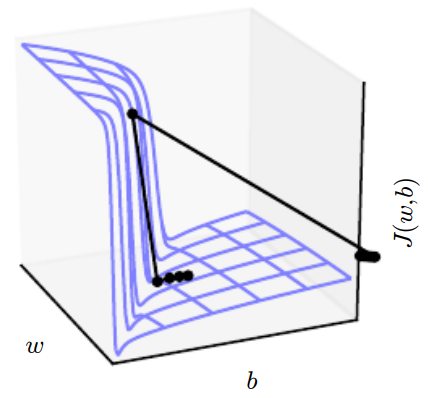
\includegraphics[width=0.4\textwidth]{Images/gard-clipping-1.png}
		\caption{The problem of large gradient value \cite{Goodfellow-et-al-2016}.}
	\end{figure}
\end{frame}

\begin{frame}{Gradient Clipping}
	\begin{itemize}
		\item Solve this problem simply by clipping gradient
		\item Two approaches to do so:
		\begin{itemize}
			\item Clipping by value
			\item Clipping by norm
		\end{itemize} 
	\end{itemize}
\end{frame}

\begin{frame}{Gradient Clipping by value}
	\begin{itemize}
		\item Set a max ($\alpha$) and min ($\beta$) threshold value
		\item For each index of gradient $\symbfit{g}_i$ if it is lower or greater than your threshold clip it:
		\[
		\begin{aligned}
			&\text{if} \; \symbfit{g}_i > \alpha: \\
			&\qquad \symbfit{g}_i \gets \alpha \\
			&\text{else if} \; \symbfit{g}_i < \beta: \\
			&\qquad \symbfit{g}_i \gets \beta
		\end{aligned}
		\]
		\item Clipping by value will not save gradient direction but still works well in practice.
		\item To preserve direction use clipping by norm.
	\end{itemize}
\end{frame}

\begin{frame}{Gradient Clipping by norm}
	\begin{itemize}
		\item Clip the norm $\|\symbfit{g}\|$ of the gradient $\symbfit{g}$ before updating parameters:
		\[
		\begin{aligned}
			&\text{if} \; \|\symbfit{g}\| > v:\\
			&\qquad \symbfit{g} \gets \frac{\symbfit g}{\|\symbfit g\|} v
		\end{aligned}
		\]
		$v$ is the threshold for clipping which is a hyperparameter.
		\item Gradient clipping saves the direction of gradient and controls its norm.
	\end{itemize}
\end{frame}

\begin{frame}{Gradient Clipping}
	\begin{itemize}
		\item The effect of gradient clipping:
	\end{itemize}
	\begin{center}
		\begin{figure}[H]
			\centering
			\begin{minipage}{0.45\textwidth}
				\centering
				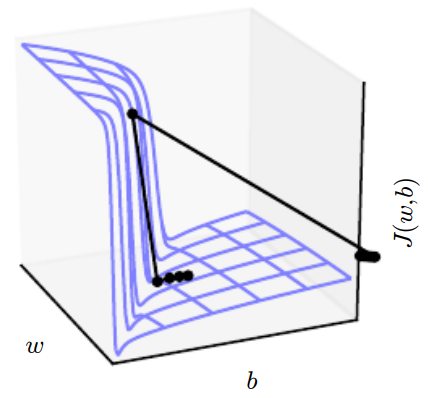
\includegraphics[width=0.8\textwidth]{Images/gard-clipping-1.png}
			\end{minipage}%\hfill
			\begin{minipage}{0.45\textwidth}
				\centering
				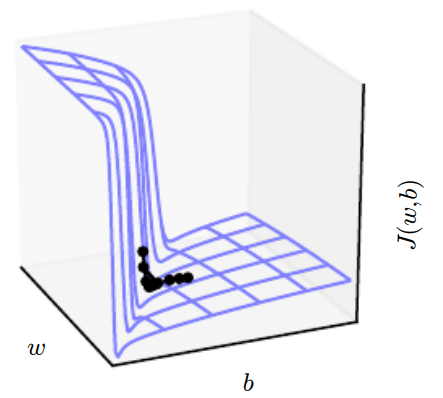
\includegraphics[width=0.8\textwidth]{Images/grad-clipping-2.png}
			\end{minipage}
			\caption{The "cliffs" landscape (left) without gradient clipping\\ and (right) with gradient clipping \cite{Goodfellow-et-al-2016}.}
		\end{figure}
	\end{center}
\end{frame}


%%%%%%%%%%%%%%%%%%%%%%%%%%%%%%%%%%%%%%%%%%%%%%%%%%%%%%%%%%%%%%%%%%%%%%%%%%%%%%%%%%
%%%%%%%%%%%%%%%%%%%%%%%%%%%%%%%%%%%%%%%%%%%%%%%%%%%%%%%%%%%%%%%%%%%%%%%%%%%%%%%%%%
\begin{frame}{Weight Initialization}
    \begin{itemize}
    	\item Is initialization really necessary?
    	\item What are the impacts of initialization?
    	\pause
%    	\item Weight initialization is critical for model performance.
    	\item A bad initialization may increase convergence time or even make optimization diverge.
    	\item How to initialize?
    	\begin{itemize}
    		\item Zero initialization
    		\item Random initialization
    	\end{itemize}
    \end{itemize}
	\begin{figure}[H]
		\centering
		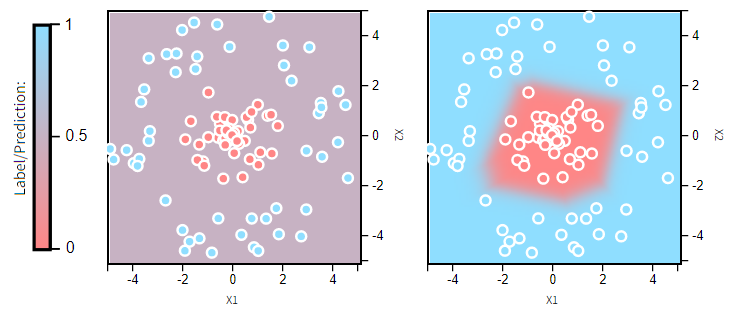
\includegraphics[width=0.65\textwidth]{Images/wi-crucial.png}
		\caption{The output of a three layer network after about 600 epoch. (left) using a bad\\ initialization method and (right) using an appropriate initialization \cite{katanforoosh-kunin}.}
	\end{figure}
\end{frame}

\begin{frame}{Weight Initialization}
	\begin{block}{Let's review some notations before we continue:}
		\begin{columns}
			\begin{column}{0.4\textwidth}
				\[
				\begin{cases}
					n^{[l]} := \text{layer $l$ neurons number}, \\
					W^{[l]} := \text{layer $l$ weights},\\
					b^{[l]} := \text{layer $l$ biases}, \\
					a^{[l]} := \text{layer $l$ outputs}
				\end{cases}
				\]
			\end{column}\hfill
			\begin{column}{0.4\textwidth}
				\begin{figure}[H]
					\centering
					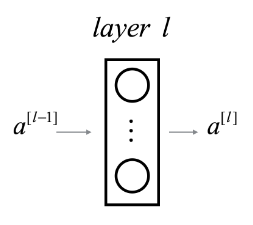
\includegraphics[width=0.65\textwidth]{Images/layer.png}
				\end{figure}
			\end{column}
		\end{columns}
	\end{block}
\end{frame}

\begin{frame}{Weight Initialization: Zero Initialization}
	\begin{block}{Zero Initialization method:}
		\[
		\begin{cases}
			W^{[l]} = \symbfit{0},\\
			b^{[l]} = \symbfit{0}
		\end{cases}
		\]
	\end{block}
	\hspace*{2em}
	\pause
	\begin{itemize}
		\item Simple but perform very poorly. (why?)
		\pause
		\item Zero initialization will lead each neuron to learn the same feature
		\item This problem is known as network {\color{red}failing to break symmetry}
		\item In fact any constant initialization suffers from this problem.
	\end{itemize}
\end{frame}

\begin{frame}{Weight Initialization: Zero Initialization}
	\begin{figure}[H]
		\centering
		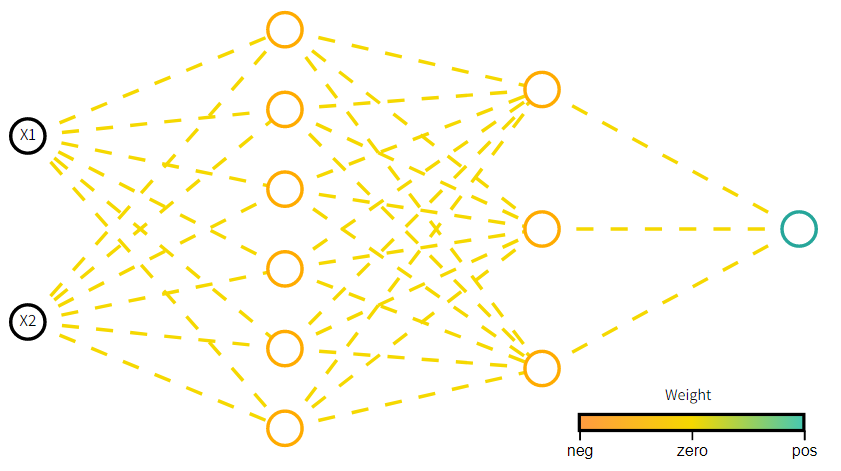
\includegraphics[width=0.65\textwidth]{Images/zero-init.png}
		\caption{As we can see network has failed to break symmetry. There has been no improvement in weights after about 600 epochs of training \cite{katanforoosh-kunin}.}
	\end{figure}
	\hspace*{2em}
	\begin{itemize}
		\item We need to break symmetry. How? using randomness.
	\end{itemize}
\end{frame}

\begin{frame}{Weight Initialization: Random Initialization}
	\begin{block}{Simple Random Initialization:}
		\[
		\begin{cases}
			W^{[l]} \sim \mathcal{N}\left(\mu=0, \sigma^2\right), \\
			b^{[l]} = 0
		\end{cases}
		\]
	\end{block}
	\hspace*{2em}
	\pause
	\begin{itemize}
		\item It depends on standard deviation ($\sigma$) value
		\item If it choose carefully, will perform well for small networks
		\item One can use $\sigma = 0.01$ as a best practice.
		\item But still has problems with deeper networks.
		\item Too small/large value for $\sigma$ will lead to vanishing/exploding gradient problem.
	\end{itemize}
\end{frame}

\begin{frame}{Weight Initialization: Random Initialization}
	\begin{figure}[H]
		\centering
		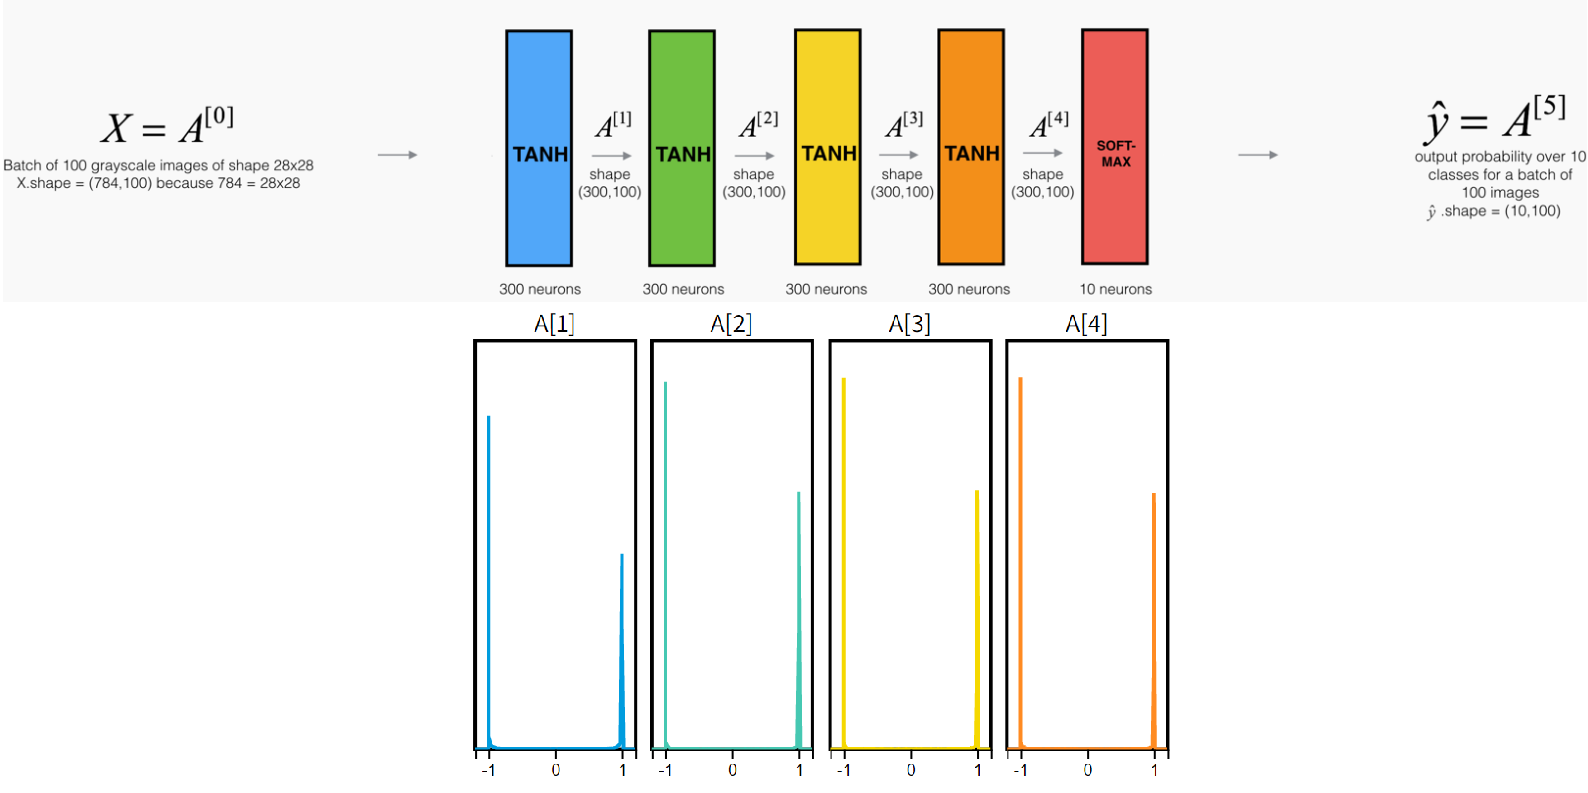
\includegraphics[width=0.9\textwidth]{Images/normal-init.png}
		\caption{The problem of normal initialization. On the top, you can see the model architecture, and on the bottom, you can see the density of each layer's output. Model has trained on MNIST dataset for 4 epoch. Weights are initialized randomly from $\mathcal{N}(0, 1)$ \cite{katanforoosh-kunin}.}
	\end{figure}
\end{frame}

\begin{frame}{Weight Initialization: Random Initialization}
	\begin{itemize}
		\item How to have a better random initialization?
		\item We need to follow these rules:
		\begin{itemize}
			\item keep the mean of the activations zero.
			\item keep the variance of the activations same across every layer.
		\end{itemize}
		\item How to do so?
	\end{itemize}
	\pause
	\hspace*{2em}
	\begin{block}{Xavier Random Initialization:}
		\[
		\begin{cases}
			W^{[l]} \sim \mathcal{N}\left(\mu=0, \sigma^2=\frac{1}{n^{[l]}}\right), \\
			b^{[l]} = 0
		\end{cases}
		\]
		{\scriptsize (this method works fine for $\tanh$, and you can read about why it works at \cite{katanforoosh-kunin}.)}
	\end{block}
\end{frame}

\begin{frame}{Weight Initialization: Random Initialization}
	\begin{figure}[H]
		\centering
		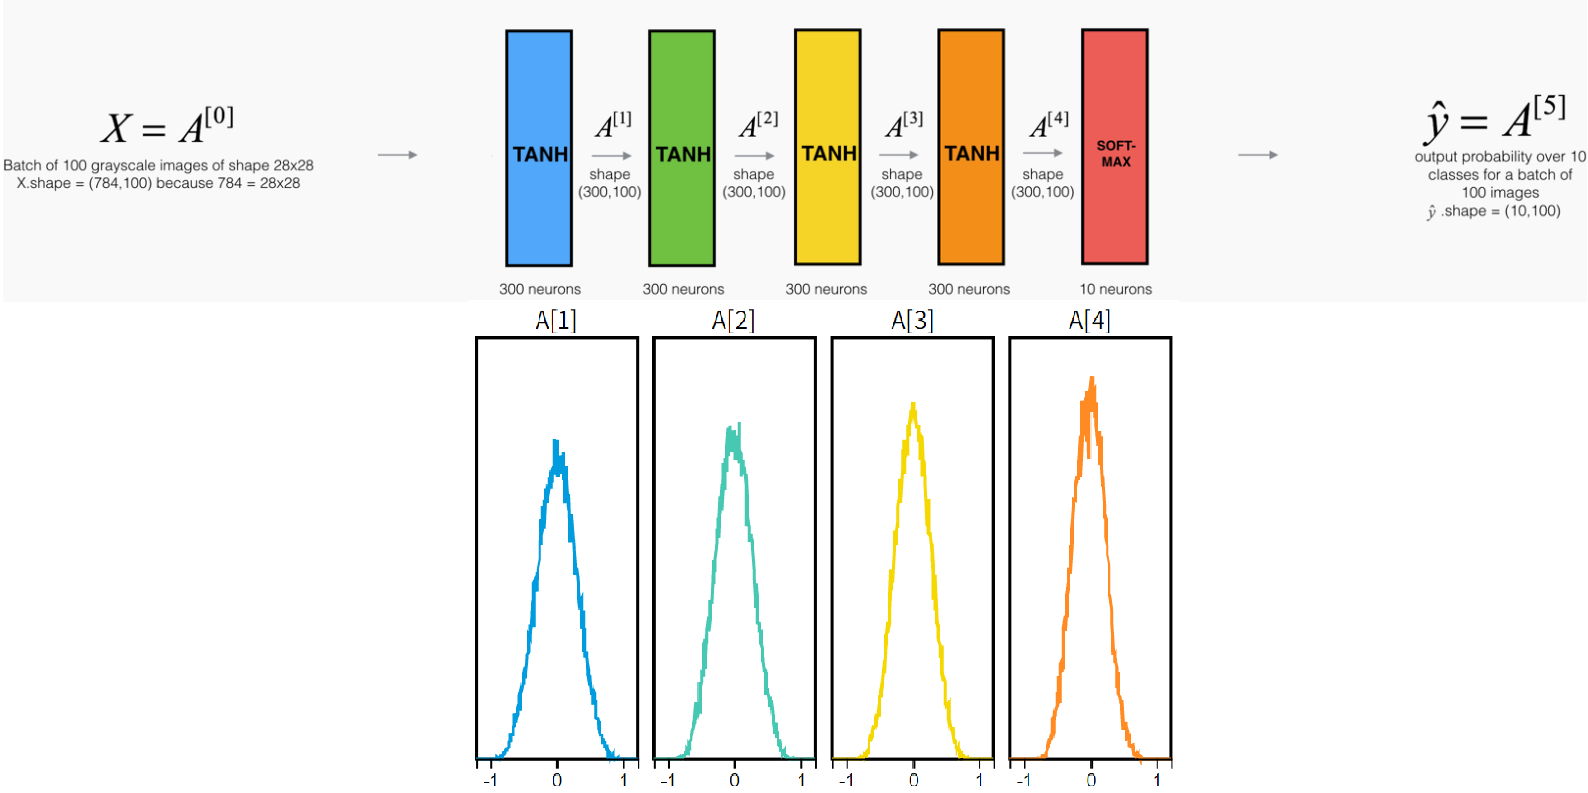
\includegraphics[width=0.9\textwidth]{Images/xavier-init.png}
		\caption{Vanishing gradient is no longer problem using Xavier initialization. Model has trained on MNIST dataset for 4 epoch. \cite{katanforoosh-kunin}.}
	\end{figure}
\end{frame}

\begin{frame}{Weight Initialization}
	\begin{itemize}
		\item We discussed weight initialization on previous slides.
		\item A god initialization will help model on vanishing/exploding gradient problem.
		\item Xavier method works well with $\tanh$ activation function.
		\begin{itemize}
			\item If you use $ReLU$ activation use He initialization:
			\begin{block}{He Initialization:}
				\setlength{\textwidth}{0.4\textwidth}
				\[
				\begin{cases}
					W^{[l]} \sim \mathcal{N}\left(\mu=0, \sigma^2=\frac{2}{n^{[l]}}\right), \\
					b^{[l]} = 0
				\end{cases}
				\]
			\end{block}
		\end{itemize}
	\end{itemize}
\end{frame}

%%%%%%%%%%%%%%%%%%%%%%%%%%%%%%%%%%%%%%%%%%%%%%%%%%%%%%%%%%%%%%%%%%%%%%%%%%%%%%%%%%
%%%%%%%%%%%%%%%%%%%%%%%%%%%%%%%%%%%%%%%%%%%%%%%%%%%%%%%%%%%%%%%%%%%%%%%%%%%%%%%%%%
\begin{frame}{Various GD types}
    
\end{frame}